%%%%%%%%%%%%%%%%%%%%%%%%%%%%%%%%%%%%%%%%%%%%%%%%%%%%%%%%%%%%%%%%%%%%%%%%%%%%
\documentclass[twocolumn,10.5pt]{article}           % pdfLaTeX の場合
\usepackage[whole]{bxcjkjatype} % whole 指定 日本語使える

\usepackage{authblk}
\usepackage[dvipdfmx]{graphicx}
\usepackage{amsmath,amssymb}
\usepackage{amsthm}
\usepackage{amsfonts}
%\usepackage{algorithmic}
\usepackage{algorithm}
\usepackage{bm}
\usepackage{color}
\usepackage{latexsym}
\bibliographystyle{junsrt}

\def\abstractname{要旨}
\def\tablename{表 }
\def\figurename{図 }
\def\indexname{索引}
\def\refname{参考文献}

\setlength{\topmargin}{-1cm}
\setlength{\textheight}{24.6cm}
\setlength{\headheight}{0cm}
\setlength{\headsep}{0cm}
\setlength{\oddsidemargin}{-1cm}
\setlength{\columnsep}{1cm}
\setlength{\textwidth}{18.5cm}
%%%%%%%%%%%%%%%%%%%%%%%%%%%%%%%%%%%%%%%%%%%%%%%%%%%%%%%%%%%%%%%%%%%%%%%%%%%

\begin{document}

% 和文タイトル
\title{Title}
\author{菊地 翔馬 \hspace{180pt} 白川 稜}
\affil{
	北海道大学大学院情報科学研究科 \hspace{50pt} 北海道大学大学院情報科学研究科\\
	kicchi@ist.hokudai.ac.jp \hspace{110pt} sira@ist.hokudai.ac.jp
}

\date{}
\maketitle

%%%%%%%%%%%%%%%%%%%%%%%%%%%%%%%%%%%%%%

\section{はじめに}
グラフはネットワークや化学構造式、
構文木など広く用いられる重要なデータ構造として知られている。
また近年ではグラフコンボリューションネットワーク(GNN)と呼ばれる
グラフデータに対する畳み込みネットワークの手法が注目を集め、
様々な分野への応用先が発見されるとともに、高いパフォーマンスを発揮している。

そこで本研究では、株価データに対して企業間の類似度を加味したグラフ構造での表現方法を提案し、
作成したグラフ上でグラフコンボリューションネットワークの手法を利用することにより、
類似企業情報を考慮した株価回帰モデルの構築法を提案する。
加えて、作成したグラフ集合において頻出クリークマイニング技術を利用することによる
ポートフォリオ作成上でのリスク分散手法も提案する。
提案手法に対して株価の実データを用いて実験を行い、その精度および有用性を評価する。

\section{データ}
\subsection{種類}
データには株価における四本値(始値、高値、安値、終値)と出来高、
またそれらの値から算出される代表的なインジケーター
(SMA、EMA、SMMA、MOMENTUM、BBAND\_UPPER、BBAND\_LOWER、MACD、MACD\_SIGNAL、
RSI、STOCH、STOCHAS\_SIGNAL、PSAR)の全17種の値を利用する。

\subsection{グラフ表現}
ここでは上記のデータに対してグラフ構造での表現方法を提案する。
まず初めに、各企業において株価のスケールが異なると類似度の評価が困難になるため、
各属性値を企業ごとに標準化し、その値を各企業の特徴ベクトルとする。
次に、各企業間の類似度の指標に各企業の特徴ベクトル間の相関係数の値を採用し、
全ての企業間での類似度を計算する。
企業$X$の特徴ベクトルが$(x_1, x_2, \cdots, x_n)$、
企業$Y$の特徴ベクトルが$(y_1, y_2, \cdots, y_n)$の時、
企業$X, Y$の類似度$(X, Y)$は以下となる。
\begin{eqnarray}
	\mbox{類似度}(X, Y) = \frac{\frac{1}{n}\sum_{i=1}^{n}(x_i - \bar{x})(y_i - \bar{y})}{\sqrt{\frac{1}{n}\sum_{i=1}^{n}(x_i - \bar{x})^2}\sqrt{\frac{1}{n}\sum_{i=1}^{n}(y_i - \bar{y})^2}}\\
	\bar{x} = \frac{1}{n}\sum_{i=1}^{n}x_i, \bar{y} = \frac{1}{n}\sum_{i=1}^{n}y_i \nonumber
\end{eqnarray}
ノードを各企業と見なし、一般的に高い相関があるとされる0.8という閾値を基準に、
類似度が閾値以上であればノード間にエッジを張るという操作を全ての企業間で行うことで
1つの無向グラフを作成する。
以上の操作を本研究でのグラフ表現方法とし、これにより作成するグラフを「相関グラフ」(図\ref{graph})と定義する。
\begin{figure}[h]
	\centering
	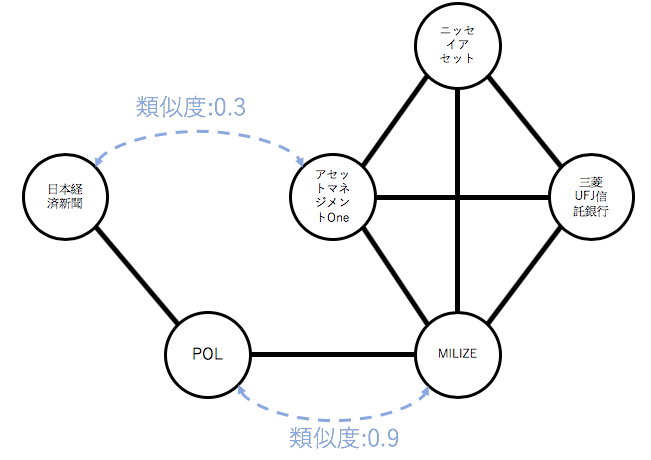
\includegraphics[width=85mm]{img/graph.png}
	\caption{相関グラフ}
	\label{graph}
\end{figure}

\section{モデル}
\subsection{GNN}
GNN は、グラフのノードとエッジに対して状態ベクトル (多次元潜在変数) を考え,非線形変換を施す。ノード毎に隣接するノードやエッジ間の情報や関係性の集約や更新を繰り返し、最終的に全ノードの状態ベク トルを集約したものをそのグラフの特徴ベクトルとする。
近年、生命科学や物質科学において化合物の物性・活性をデータ駆動方式で予測する手法として様々なアルゴリズムの研究がされている。本研究では、2.2の方法で生成された相関グラフに対して行う畳み込み操作を提案した。
\subsubsection{畳み込み操作}
グラフ構造データは、基本的にサイズが異なることがあり、通常、入力サイズの異なるデータはニューラルネットワークへの入力に適さない。そこで今回は、あるノードに対して、隣接しているノードの数に応じて計算する方法をとることで、任意の形のグラフの入力に対応した。あるノードとそれに隣接するノードの畳み込みは図\ref{conv}のように行う。
これをすべてのノードについて行い、これを複数回行うことで、隣接するノードの情報を持つ特徴ベクトルを計算する。
\begin{figure}[htbp]
	\centering
	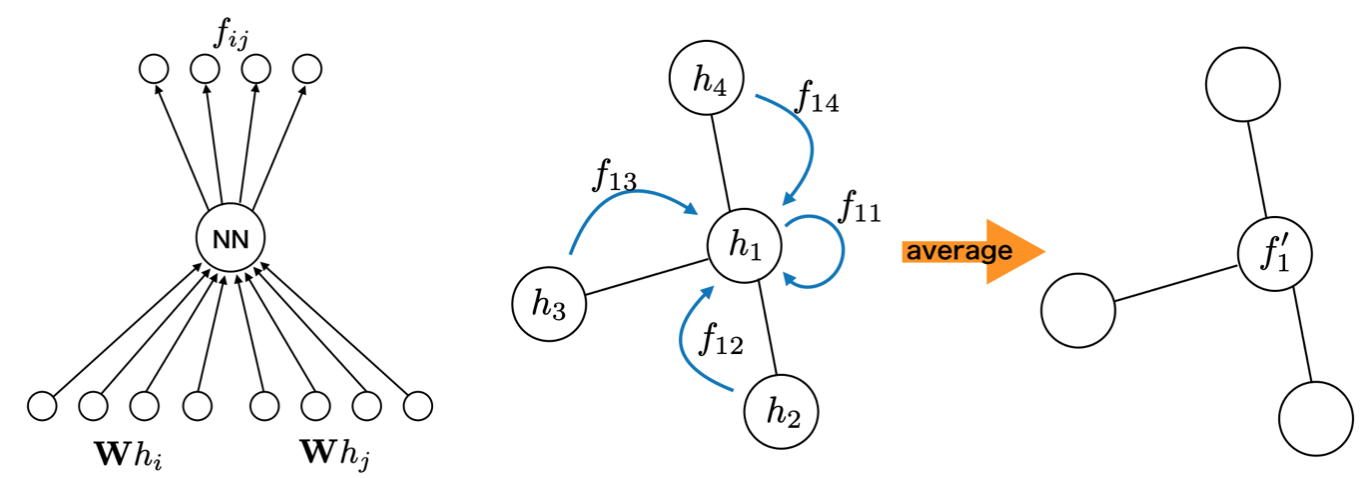
\includegraphics[width=85mm]{img/img02.png}
	\caption{左図:隣接するノードと自分のノードのベクトルを線形変換した後に連結し単純ニューラルネットワークに通す。右図:隣接するノード全てに対して、左図の操作をした後、それらの平均を取ったものをノードの新しいベクトルとする。}
	\label{conv}
\end{figure}
\subsection{頻出クリークマイニング}
ここではポートフォリオ作成時のリスク分散について考える。
株価というものは非常に繊細であり、それまでの株価の値動きからだけでは予測できない場合が存在する。
例を挙げるとリーマンショックやITバブルなど、世界全体もしくは一部業界の株価が急激に変動することがある。
こういったケースを考慮すると、一部の業界のみでポートフォリオを作成することはリスク分散の観点から見ると良いものではない。
複数の業界からポートフォリオを作成する場合の方が、一部業界の株価が暴落した際にも対応しやすい。
しかし株価というものは同時にすごく複雑なもので、業界が同じだからといって同じ値動きをするとは限らない、
むしろ違う業界の企業間で似た動きをするものも存在する。

この点に関して、本研究ではグラフの頻出クリーク構造という点に着目してリスク分散に対するアプローチを取る。
グラフの頻出クリーク構造とは複数グラフに出現するクリーク構造のことを刺し、
ここで扱うグラフは類似度を表現するため、値動きが類似している回数が多く見られる企業の集合を表す。
本提案では頻出度50\%以上の企業集合に関しては、
1つの企業しかポートフォリオに採用しないことでリスク分散を図る。

(注:このリスク分散の提案に関しては計算時間の都合上結果に反映されていない)

\section{実験&結果}
\subsection{データセット}
日経225(2019.02.10時点)の週足の株価データ2016から2018の3年分のデータを扱う。
また目的変数は、(本コンペティションの問題設定上)説明変数に対応する時刻の三週間後の終値とする。

\subsection{実験}
hoge
\subsection{結果}
hoge

\section{考察}
hoge

\section{展望}
edgeの重みを考慮したバージョン\\
回帰にRNNを使う、各企業ごとに(R)NNをフィッティング\\
計算時間を考慮すると、グラフ全体で特徴ベクトル生成$\to$回帰

\bibliography{ref}

%%%%%%%%%%%%%%%%%%%%%%%%%%%%%%%%%%%%%%

\end{document}
